\documentclass[tikz=true]{standalone}
\begin{document}
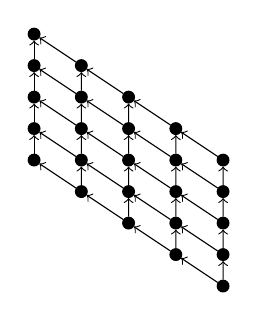
\begin{tikzpicture}
  % DOM
  \begin{scope}[xscale=0.6, yscale=0.4, every node/.style={draw, shape=circle, fill=black, inner sep=1.5pt}]
    \node (n04) at (0,4) {};
    \node (n05) at (0,5) {};
    \node (n06) at (0,6) {};
    \node (n07) at (0,7) {};
    \node (n08) at (0,8) {};

    \node (n13) at (1,3) {};
    \node (n14) at (1,4) {};
    \node (n15) at (1,5) {};
    \node (n16) at (1,6) {};
    \node (n17) at (1,7) {};

    \node (n22) at (2,2) {};
    \node (n23) at (2,3) {};
    \node (n24) at (2,4) {};
    \node (n25) at (2,5) {};
    \node (n26) at (2,6) {};

    \node (n31) at (3,1) {};
    \node (n32) at (3,2) {};
    \node (n33) at (3,3) {};
    \node (n34) at (3,4) {};
    \node (n35) at (3,5) {};

    \node (n40) at (4,0) {};
    \node (n41) at (4,1) {};
    \node (n42) at (4,2) {};
    \node (n43) at (4,3) {};
    \node (n44) at (4,4) {};

    % Straight
    \draw[->] (n04) edge (n05);
    \draw[->] (n05) edge (n06);
    \draw[->] (n06) edge (n07);
    \draw[->] (n07) edge (n08);

    \draw[->] (n13) edge (n14);
    \draw[->] (n14) edge (n15);
    \draw[->] (n15) edge (n16);
    \draw[->] (n16) edge (n17);

    \draw[->] (n22) edge (n23);
    \draw[->] (n23) edge (n24);
    \draw[->] (n24) edge (n25);
    \draw[->] (n25) edge (n26);

    \draw[->] (n31) edge (n32);
    \draw[->] (n32) edge (n33);
    \draw[->] (n33) edge (n34);
    \draw[->] (n34) edge (n35);

    \draw[->] (n40) edge (n41);
    \draw[->] (n41) edge (n42);
    \draw[->] (n42) edge (n43);
    \draw[->] (n43) edge (n44);

    % Crossing
    \draw[->] (n40) edge (n31);
    \draw[->] (n31) edge (n22);
    \draw[->] (n22) edge (n13);
    \draw[->] (n13) edge (n04);

    \draw[->] (n41) edge (n32);
    \draw[->] (n32) edge (n23);
    \draw[->] (n23) edge (n14);
    \draw[->] (n14) edge (n05);

    \draw[->] (n42) edge (n33);
    \draw[->] (n33) edge (n24);
    \draw[->] (n24) edge (n15);
    \draw[->] (n15) edge (n06);

    \draw[->] (n43) edge (n34);
    \draw[->] (n34) edge (n25);
    \draw[->] (n25) edge (n16);
    \draw[->] (n16) edge (n07);

    \draw[->] (n44) edge (n35);
    \draw[->] (n35) edge (n26);
    \draw[->] (n26) edge (n17);
    \draw[->] (n17) edge (n08);
  \end{scope}
\end{tikzpicture}
\end{document}
